\achapter{21}{Complex Eigenvalues} \label{sec:complex_eigenvalues}

\vspace*{-17 pt}
\framebox{
\parbox{\dimexpr\linewidth-3\fboxsep-3\fboxrule}
{\begin{fqs}
\item What properties do complex eigenvalues of a real matrix satisfy?
\item What properties do complex eigenvectors of a real matrix satisfy?
\item What is a rotation-scaling matrix?
\item How do we find a rotation-scaling matrix within a matrix with complex eigenvalues?
\end{fqs}}}% \hspace*{3 pt}}

\vspace*{13 pt}

\csection{Application: The Gershgorin Disk Theorem}

We have now seen different methods for calculating/approximating eigenvalues of a matrix. The algebraic method using the characteristic polynomial can provide exact values, but only in cases where the size of the matrix is small. Methods like the power method allow us to approximate eigenvalues in many, but not all, cases. These approximation techniques can be made more efficient if we have some idea of where the eigenvalues are. The Gershgorin Disc Theorem is a useful tool that can quickly provide bounds on the location of eigenvalues using elementary calculations. For example, using the Gershsgorin Disk Theorem we can quickly tell that the real parts of the eigenvalues of the matrix 
\[\left[ \begin{array}{ccr} 3&1&-1 \\ 0&-1+i&i \\ 2&1&-2i \end{array} \right]\]
lie between $-4$ and 5 and the imaginary parts lie between $-5$ and 2. Even more, we can say that the eigenvalues lie in the disks (called \emph{Gershgorin disks}) shown in Figure \ref{F:Gershgorin_1}.
\begin{figure}[ht]
\begin{center}
\resizebox{!}{2.5in}{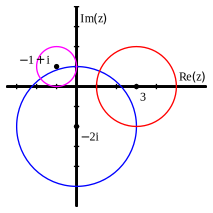
\includegraphics{Gershgorin_1.eps}}
\end{center}
\caption{Gershgorin disks.}
\label{F:Gershgorin_1}
\end{figure}
We will learn more details about the Gershgorin Disk Theorem at the end of this section. 

\csection{Introduction}

So far we have worked with real matrices whose eigenvalues are all real. However, the characteristic polynomial of a matrix with real entries can have complex roots. In this section we investigate the properties of these complex roots and their corresponding eigenvectors, how these complex eigenvectors are found, and the geometric interpretation of the transformations defined by matrices with complex eigenvalues. Although we can consider matrices that have complex numbers as entries, we will restrict ourselves to matrices with real entries. 

\begin{pa} \label{pa:4_e} Let $A = \left[ \begin{array}{rc} 2&4 \\ -2&2 \end{array} \right]$.
	\be
	\item Find the characteristic polynomial of $A$.

	\item Find the eigenvalues of $A$. You should get two complex numbers. How are these complex numbers related?

	\item Find an eigenvector corresponding to each eigenvalue of $A$. You should obtain vectors with complex entries.

	\ee
\end{pa}

\csection{Complex Eigenvalues}

As you noticed in Preview Activity \ref{pa:4_e}, the complex roots of the characteristic equation of a real matrix $A$ come in complex conjugate pairs. This should come as no surprise since we know through our use of the quadratic formula that complex roots of (real) quadratic polynomials come in complex conjugate pairs. More generally, if $p(x)=a_0+a_1x+a_2x^2 + \cdots + a_nx^n$ is a polynomial with real coefficients and $z$ is a root of this polynomial, meaning $p(z)=0$, then 
\[ 0=\overline{p(z)} = \overline{a_0+a_1z+a_2z^2 + \cdots + a_nz^n} = a_0 + a_1 \overline{z} + a_2 \overline{z}^2 + \cdots + a_n \overline{z}^n = p(\overline{z})\, .\]
Therefore, $\overline{z}$ is also a root of $p(x)$.

\begin{activity} \label{act:4e_1} Let $A=\left[ \begin{array}{cr} 0&-1 \\ 1&0 \end{array} \right]$. 

	\ba
	\item The matrix transformation $T:\R^2 \to \R^2$ defined by $T(\vx)=A\vx$ is a rotation transformation. What is the angle of rotation?
	
	
	
	\item Find the eigenvalues of $A$. For each eigenvalue, find an eigenvector.

	
		
	\ea
\end{activity}



In Preview Activity \ref{pa:4_e} and in Activity \ref{act:4e_1}, you found that if $\vv$ is an eigenvector of $A$ corresponding to $\lambda$, then $\overline{\vv}$ obtained by taking the complex conjugate of each entry in $\vv$ is an eigenvector of $A$ corresponding to $\overline{\lambda}$. Specifically, if $\vv=\vu+i\vw$ where both $\vu$ and $\vw$ are real vectors is an eigenvector of $A$, then so is $\overline{\vv} = \vu-i\vw$. We can justify this property using matrix algebra as follows:
\[ A\overline{\vv} = \overline{A}\overline{\vv} = \overline{A\vv} = \overline{\lambda \vv} = \overline{\lambda} \overline{\vv} \, .\]
In the first equality, we used the fact that $A$ is a real matrix, so $\overline{A}=A$. In all the other equalities, we used the properties of the conjugation operation in complex numbers.

\csection{Rotation and Scaling Matrices}

Recall that a rotation matrix is of the form 
\[ R_\theta= \left[ \begin{array}{cr} \cos(\theta)&-\sin(\theta) \\ \sin(\theta)&\cos(\theta) \end{array} \right]\]
where the rotation is counterclockwise about the origin by an angle of $\theta$ radians. In Activity \ref{act:4e_1}, we considered the rotation matrix with angle $\pi/2$ in counterclockwise direction. We will soon see that rotation matrices play an important role in the geometry of a matrix transformation for a matrix that has complex eigenvalues. In this activity, we will restrict ourselves to the $2 \times 2$ case, but similar arguments can be made in higher dimensions.



\begin{activity} \label{act:4e_2} Let $A=\left[ \begin{array}{rc} 1&1 \\ -1&1 \end{array} \right]$. 

	\ba
	\item Explain why $A$ is not a rotation matrix.
	
	
	
	\item Although $A$ is not a rotation matrix, there is a rotation matrix $B$ inside $A$. To find the matrix $B$, factor out $\sqrt{2}$ from all entries of $A$. In other words, write $A$ as a product of two matrices in the form
\[ A = \left[ \begin{array}{cc} \sqrt{2} &0 \\ 0&\sqrt{2} \end{array} \right] B \;. \]
		
	
		
	\item The $B$ matrix is a rotation matrix with an appropriate $\theta$. Find this $\theta$.
	
	
	
	\item If we think about the product of two matrices as applying one transformation after another, describe the effect of the matrix transformation defined by $A$ geometrically. 

	 		
			
	\ea
\end{activity}



More generally, if we have a matrix $A$ of the form $A=\left[ \begin{array}{cr} a&-b \\ b&a \end{array} \right]$, then 
\[ A = \left[ \begin{array}{cc} \sqrt{a^2+b^2} &0 \\ 0&\sqrt{a^2+b^2} \end{array} \right] \left[ \begin{array}{cc} \frac{a}{\sqrt{a^2+b^2}}&\frac{-b}{\sqrt{a^2+b^2}} \\ \frac{b}{\sqrt{a^2+b^2}}&\frac{a}{\sqrt{a^2+b^2}}\end{array} \right] \, .\]
The first matrix in the decomposition is a scaling matrix with a scaling factor of $s=\sqrt{a^2+b^2}$. So if $s>1$, the transformation stretches vectors, and if $s<1$, the transformation shrinks vectors. The second matrix in the decomposition is a rotation matrix with angle $\theta$ such that $\cos(\theta)=\frac{a}{\sqrt{a^2+b^2}}$ and $\sin(\theta)=\frac{b}{\sqrt{a^2+b^2}}$. This angle is also the angle between the positive $x$-axis and the vector $\vv=\left[ \begin{array}{c} a\\ b\end{array} \right]$. We will refer to the matrices of the form $\left[ \begin{array}{cr} a&-b \\ b&a \end{array} \right]$ as \emph{rotation-scaling matrices}\index{rotation-scaling matrices}. 

\csection{Matrices with Complex Eigenvalues}

Now we will investigate how a general $2\times 2$ matrix with complex eigenvalues can be seen to be similar (both in a linear algebra and a colloquial meaning) to a rotation-scaling matrix.



\begin{activity} \label{act:4e_3} Let $B=\left[ \begin{array}{cr} 1&-5\\2&3 \end{array} \right]$. The eigenvalues of $B$ are $2\pm 3i$.  An eigenvector for the eigenvalue $2-3i$ is $\vv=\left[ \begin{array}{c} -5 \\ 1-3i\end{array} \right]$. We will use this eigenvector to show that $B$ is similar to a rotation-scaling matrix.

	\ba
	\item Any complex vector $\vv$ can be written as $\vv=\vu+i\vw$ where both $\vu$ and $\vw$ are real vectors. What are these real vectors $\vu$ and $\vw$ for the eigenvector $\vv$ above?
	
	
	
	\item Let $P=[ \vu \ \vw ]$ be the matrix whose first column is the real part of $\vv$ and whose second column is the imaginary part of $\vv$ (without the $i$). Find $R=P^{-1}BP$.
		
	
		
	\item Express $R$ as a product of a rotation and a scaling matrix. What is the factor of scaling? What is the rotation angle?
	
	
				
	\ea
\end{activity}



In Activity \ref{act:4e_3}, we saw that the matrix $B$ with complex eigenvalues $2\pm 3i$ is similar to a rotation-scaling matrix. Specifically $R=P^{-1}BP$, where the columns of $P$ are the real and imaginary parts of an eigenvector of $B$, is the rotation-scaling matrix with a factor of scaling by $\sqrt{2^2+3^2}$ and a rotation by angle $\theta=\arccos(\frac{2}{\sqrt{2^2+3^2}})$. 



Does a similar decomposition result hold for a general $2\times 2$ matrix with complex eigenvalues? We investigate this question in the next activity.



\begin{activity} \label{act:4e_4} Let $A$ be a $2\times 2$ matrix with complex eigenvalue $\lambda=a-bi$, $b\neq 0$, and corresponding complex eigenvector $\vv=\vu+i\vw$.

	\ba
	\item Explain why $A\vv = A\vu+iA\vw$.
	
	
	\item Explain why $\lambda\vv = (a\vu+b\vw)+i (a\vw-b\vu)$.
		
	
		
	\item Use the previous two results to explain why 
	\begin{itemize}
	\item $A\vu=a\vu+b\vw$ and 
	\item $A\vw = a\vw - b\vu$.
	\end{itemize}
	
	
	
	\item Let $P=[ \vu \ \vw ]$. We will now show that $AP=PR$ where $R=\left[ \begin{array}{cr} a&-b \\ b&a \end{array} \right]$.
	
	\begin{enumerate}[i.]
	\item Without any calculation, explain why
\[AP = [ A\vu \  A\vw ].\]



	\item Recall that if $M$ is an $m \times n$ matrix and $\vx$ is an $n \times 1$ vector, then the matrix product $M\vx$ is a linear combination of the columns of $M$ with weights the corresponding entries of the vector $\vx$. Use this idea to show that
\[PR = [ a\vu + b\vw \  -b\vu + a\vw ].\]



	\item Now explain why $AP = PR$.
	
	
	
	\item Assume for the moment that $P$ is an invertible matrix. Show that $A = PRP^{-1}$.
	
	
	
	\end{enumerate}
				
	\ea
\end{activity}



Your work in Activity \ref{act:4e_4} shows that any $2\times 2$ matrix is similar to a rotation-scaling matrix with a factor of scaling by $\sqrt{a^2+b^2}$ and a rotation by angle $\theta=\arccos(\frac{a}{\sqrt{a^2+b^2}})$ if $b\geq 0$, and $\theta=-\arccos(\frac{a}{\sqrt{a^2+b^2}})$ if $b<0$. Geometrically, this means that every $2 \times 2$ real matrix with complex eigenvalues is just a scaled rotation ($R$) with respect to the basis $\B$ formed by $\vu$ and $\vw$ from the complex eigenvector $\vv$. Multiplying by $P^{-1}$ and $P$ simply provides the change of basis from the standard basis to the basis $\B$, as we will see in detail when we learn about linear transformations.



\begin{theorem} Let $A$ be a real $2\times 2$ matrix with complex eigenvalue $a-bi$ and corresponding eigenvector $\vv=\vu+i\vw$. Then 
\[ A=PRP^{-1} \; , \text{ where } P=[ \vu \ \vw ] \; \text{ and } R= \left[ \begin{array}{cr} a&-b \\ b&a \end{array} \right] \, .\]
\end{theorem}



The one fact that we have not yet addressed is why the matrix $P = [ \vu \ \vw ]$ is invertible. We do that now to complete the argument.

Let $A$ be a real $2 \times 2$ matrix with $A \vv = \lambda \vv$, where $\lambda = a-bi$, $b \neq 0$ and $\vv=\vu+i\vw$ (where $\vu$ and $\vv$ are in $\R^2$) with $\vw \neq \vzero$. From Activity \ref{act:4e_4} we know that 
\[A\vu = a\vu + b\vw \ \text{ and } \ A\vw = a\vw - b \vu.\]

To show that $\vu$ and $\vw$ are linearly independent, we need to show that no nontrivial linear combination of $\vu$ and $\vw$ can be the zero vector. Suppose
\[x_1\vu + x_2\vw = \vzero\]
for some scalars $x_1$ and $x_2$. We will show that $x_1 = x_2 = 0$. Assume to the contrary that one of $x_1, x_2$ is not zero. First, assume $x_1 \neq 0$. Then $\vu = -\frac{x_2}{x_1} \vw$. Let $c = -\frac{x_2}{x_1}$. From this we have
\begin{align*}
A \vu &= A(c\vw) \\
A \vu &= cA \vw \\
a\vu + b\vw &= c(a \vw - b \vu) \\
(a+cb)\vu &= (ca-b)\vw \\
(a+cb)(c\vw) &= (ca-b)\vw.
\end{align*}
Since $\vw \neq \vzero$ we must have $(a+cb)c = ca-b$. A little algebra shows that $(c^2+1)b = 0$. Since $b \neq 0$, we conclude that $c^2+1=0$, which is impossible for a real constant $c$. Therefore, we cannot have $x_1 \neq 0$. A similar argument (left to the reader) shows that $x_2 = 0$. Thus we can conclude that $\vu$ and $\vw$ are linearly independent.

\csection{Examples}

\ExampleIntro

\begin{example} Let $A = \left[ \begin{array}{rcr} 0&1&0 \\ -1&0&-1 \\ 1&1&1 \end{array} \right]$.
\ba
\item Without doing any computations, explain why not all of the eigenvalues of $A$ can be complex.

\item Find all of the eigenvalues of $A$.

\ea

\ExampleSolution
\ba
\item Since complex eigenvalues occur in conjugate pairs, the complex eigenvalues with nonzero imaginary parts occur in pairs. Since $A$ can have at most 3 different eigenvalues, at most two of them can have nonzero imaginary parts. So at least one eigenvalue of $A$ is real. 

\item For this matrix $A$ we have $A - \lambda I_3 = \left[ \begin{array}{rrc} -\lambda&1&0 \\ -1&-\lambda&-1 \\ 1&1&-\lambda+1 \end{array} \right]$. Using a cofactor expansion along the first row gives us 
\begin{align*}
\det(A - \lambda I_3) &= (-\lambda)\left((-\lambda)(1-\lambda)+1\right) - \left((-1)(1-\lambda)+1\right) \\
	&= -\lambda^3 + \lambda^2 - \lambda +1 - \lambda -1 \\
	&= \lambda^3 + \lambda^2 - 2\lambda \\
	&= -\lambda(\lambda^2 -\lambda + 2).
\end{align*}
The roots of the characteristic polynomial are $\lambda = 0$ and 
\[\lambda = \frac{1 \pm \sqrt{1-4(2)}}{2} = \frac{1}{2}(1 \pm \sqrt{7}i).\]


\ea


\end{example}

\begin{example} Let $A = \left[ \begin{array}{rc} 1&2\\-1&3 \end{array} \right]$.  Find a rotation scaling matrix $R$ that is similar to $A$. Identify the rotation and scaling factor.


\ExampleSolution
The eigenvalues of $A$ are the roots of the characteristic polynomial
\begin{align*}
p(\lambda) &= \det(A - \lambda I_2) \\
	&= \det\left(\left[ \begin{array}{rc} 1-\lambda&2\\-1&3-\lambda \end{array} \right]\right) \\
	&= (1-\lambda)(3-\lambda) + 2 \\
	&= \lambda^2 -4\lambda + 5.
\end{align*}
The quadratic formula shows that the roots of $p(\lambda)$ are 
\[\frac{4 \pm \sqrt{-4}}{2} = 2 \pm i.\]
To find an eigenvector for $A$ with eigenvalue $2-i$, we row reduce 
\[A - (2-i) I_3 =   \left[ \begin{array}{cc} -1+i&2\\-1&1+i \end{array} \right]\]
to 
\[\left[ \begin{array}{cc} 1&-i-1\\0&0 \end{array} \right].\]
An eigenvector for $A$ with eigenvalue $2-i$ is then 
\[[ 1+i \  \ 1]^{\tr} = [1 \ 1]^{\tr} + i[1 \ 0]^{\tr}.\]
Letting $P = \left[  \begin{array}{cc} 1&1\\1&0 \end{array} \right]$, we have 
\[R = P^{-1}AP = \left[ \begin{array}{cr} 2&-1\\1&2 \end{array} \right].\]
The scaling is determined by the determinant of $R$ which is $5$, and the angle $\theta$ of rotation satisfies $\sin(\theta) = \frac{1}{5}$. This makes  $\theta \approx 0.2014$ radians or approximately $11.5370^{\circ}$ counterclockwise. 


\end{example}



\csection{Summary}

\begin{itemize}
\item For a real matrix, complex eigenvalues appear in conjugate pairs. Specifically, if $\lambda=a+ib$ is an eigenvalue of a real matrix $A$, then $\overline{\lambda}=a-ib$ is also an eigenvalue of $A$.
\item For a real matrix, if a $\vv$ is an eigenvector corresponding to $\lambda$, then the vector $\overline{\vv}$ obtained by taking the complex conjugate of each entry in $\vv$ is an eigenvector corresponding to $\overline{\lambda}$.
\item The rotation-scaling matrix $A=\left[ \begin{array}{cr} a&-b \\ b&a \end{array} \right]$ can be written as 
\[ \left[ \begin{array}{cc} \sqrt{a^2+b^2} &0 \\ 0&\sqrt{a^2+b^2} \end{array} \right] \left[ \begin{array}{cc} \frac{a}{\sqrt{a^2+b^2}}&\frac{-b}{\sqrt{a^2+b^2}} \\ \frac{b}{\sqrt{a^2+b^2}}&\frac{a}{\sqrt{a^2+b^2}}\end{array} \right] \, .\]
This decomposition geometrically means that the transformation corresponding to $A$ can be viewed as a rotation by angle $\theta=\arccos\left(\frac{a}{\sqrt{a^2+b^2}}\right)$ if $b\geq 0$, or $\theta=-\arccos\left(\frac{a}{\sqrt{a^2+b^2}}\right)$ if $b<0$, followed by a scaling by factor $\sqrt{a^2+b^2}$. 
\item If $A$ is a real $2\times 2$ matrix with complex eigenvalue $a-bi$ and corresponding eigenvector $\vv=\vu+i\vw$, then $A$ is similar to the rotation-scaling matrix $R=\left[ \begin{array}{cr} a&-b \\ b&a \end{array} \right]$. More specifically,
\[ A=PRP^{-1} \; , \text{ where } P=[ \vu \ \vw ]\, .\]
\end{itemize}


\csection{Exercises}
\be
\item Find eigenvalues and eigenvectors of each of the following matrices.
\ba \item $\left[ \begin{array}{rc} 2&4 \\ -2&2 \end{array} \right]$
\item $\left[ \begin{array}{rc} 3&2 \\ -1&1 \end{array} \right]$
\item $\left[ \begin{array}{cr} 1&-2 \\ 4&-3 \end{array} \right]$
\ea

\item Find a rotation-scaling matrix where the rotation angle is $\theta=3\pi/4$ and scaling factor is less than 1.

\item Determine which rotation-scaling matrices have determinant equal to 1. Be as specific as possible.

\item Determine the rotation-scaling matrix inside the matrix $\left[ \begin{array}{rc} 2&4 \\ -2&2 \end{array} \right]$.

\item Find a real $2\times 2$ matrix with eigenvalue $1+2i$.

\item Find a real $2\times 2$ matrix which is not a rotation-scaling matrix with eigenvalue $-1+2i$.

\item We have seen how to find the characteristic polynomial of an $n \times n$ matrix. In this exercise we consider the reverse question. That is, given a polynomial $p(\lambda)$ of degree $n$, can we find an $n \times n$ matrix whose characteristic polynomial is $p(\lambda)$? 
\ba
\item Find the characteristic polynomial of the $2 \times 2$ matrix $C = \left[ \begin{array}{cc} 0&-a_0\\1&-a_1 \end{array} \right]$. Use this result to find a real valued matrix whose eigenvalues are $1+i$ and $1-i$. 

\item Repeat part (a) by showing that $p(\lambda) = -\left(\lambda^3+a_2\lambda^2+a_1\lambda+a_0\right)$ is the characteristic polynomial of the $3 \times 3$ matrix $C = \left[ \begin{array}{ccc} 0&0&-a_0\\1&0&-a_1\\0&1&-a_2 \end{array} \right]$.  

\item We can generalize this argument. Prove, using mathematical induction, that the polynomial
\[p(\lambda) =(-1)^n\left( \lambda^n + a_{n-1}\lambda^{n-1} + a_{n-2}\lambda^{n-2} + \cdots + a_1 \lambda + a_0\right)\]
is the characteristic polynomial of the matrix 
\[C = \left[ \begin{array}{cccccc} 0&0&0&\cdots&0&-a_{0}\\
1&0&0&\cdots&0&-a_{1} \\
0&1&0&\cdots&0&-a_2 \\
\vdots & \vdots &\vdots& \ddots & \vdots   & \vdots   \\
0 & 0 & 0& \cdots &  1 & -a_{n-1} 
\end{array} \right].\]
The matrix $C$ is called the \emph{companion matrix}\index{companion matrix} for $p(\lambda)$.

\ea


\item Label each of the following statements as True or False. Provide justification for your response.
\ba
\item \textbf{True/False} If $3-4i$ is an eigenvalue of a real matrix, then so is $3+4i$.

\item \textbf{True/False} If $2+3i$ is an eigenvalue of a $3\times 3$ real matrix $A$, then $A$ has three distinct eigenvalues.

\item \textbf{True/False} Every $2\times 2$ real matrix with complex eigenvalues is a rotation-scaling matrix.

\item \textbf{True/False} Every square matrix with real entries has real number eigenvalues. 

\item \textbf{True/False} If $A$ is a $2\times 2$ matrix with complex eigenvalues similar to a rotation-scaling matrix $R$, the eigenvalues of $A$ and $R$ are the same.

\item \textbf{True/False} If $A$ is a real matrix with complex eigenvalues, all eigenvectors of $A$ must be non-real.


\ea

\ee

\csection{Project: Understanding the Gershgorin Disk Theorem}

To understand the Gershgorin Disk Theorem, we need to recall how to visualize a complex number in the plane. Recall that a complex number $z$ is a number of the form $z = a+bi$ where $a$ and $b$ are real numbers and $i^2 = -1$. The number $a$ is the real part of $z$, denoted as $\text{Re}(z)$, and $b$ is the imaginary part of $z$, denoted $\text{Im}(z)$. The set of all complex numbers is denoted $\C$. We define addition and multiplication on $\C$ as follows. For $a+bi, c+di \in \C$, 
\[(a+bi) + (c+di) = (a+c) + (b+d)i \ \ \ \ \ \text{and} \ \ \ \ \ (a+bi)(c+di) = (ac-bd) + (ad+bc)i.\]
Note that the product is what we would expect if we ``expanded" the product in the normal way and used the fact that $i^2=-1$. The set of complex numbers forms a field -- that is, $\C$ satisfies all of the same properties as $\R$ as stated in Theorem \ref{thm:1_d_reals}. 

We can visualize the complex number $a+bi$ in the plane as the point $(a,b)$. Here we are viewing the horizontal axis as the real axis and the vertical axis as the imaginary axis. The length (or magnitude) of the complex number $z = a+bi$, which we denote as $|z|$, is the distance from the origin to $z$. So by the Pythagorean Theorem we have $|a+bi| = \sqrt{a^2+b^2}$. Note that the magnitude of $z = a+bi$ can be written as a complex product 
\[|z| = \sqrt{(a+bi)(a-bi)}.\]
The complex number $a-bi$ is called the \emph{complex conjugate} of $z=a+bi$ and is denoted as $\overline{z}$. A few important properties of real numbers and their conjugates are the following. Let $z = a+bi$ and $w = c+di$ be complex numbers. Then

\begin{itemize}
\item $\overline{z+w} = \overline{(a+c) + (b+d)i} = (a+c)-(b+d)i = (a-bi) + (c-di) = \overline{z} + \overline{w}$,
\item $\overline{zw} = \overline{(ac-bd) + (ad+bc)i} = (ac-bd)-(ad+bc)i = (a-bi)(c-di) = \overline{z} \overline{w}$,
\item $\overline{\overline{z}} = z$,
%\item $\Re(z\overline{w}) = \Re((ac+bd) + (bc-ad)i) = ac+bd$,
%\item $\Im(z\overline{w}) = bc-ad$,
\item $|z| = \sqrt{a^2+b^2} \geq \sqrt{a^2} = |a| = |\text{Re}(z)|$,
\item $|z| = \sqrt{a^2+b^2} \geq \sqrt{b^2} = |b| = |\text{Im}(z)|$,
\item $\left| \overline{z} \right| = |z|$,
\item $|z| = 0$ if and only if $z = 0$,
\item If $p(x)$ is a polynomial with real coefficients and the complex number $z$ satisfies $p(z) = 0$, then $p\left(\overline{z}\right) = 0$ as well. 
\end{itemize}

Using these facts we can show that the triangle inequality is true for complex numbers. That is, 
\[|z+w| \leq |z| + |w|.\]
To see why, notice that 
\begin{align*}
|z+w|^2 &= (z+w)(\overline{z+w}) \\
	&= (z+w)(\overline{z} + \overline{w}) \\
	&= z\overline{z} + z\overline{w} + w \overline{z} + w \overline{w} \\
	&= z\overline{z} + z\overline{w} + \overline{zw\overline{w}} + w \overline{w} \\
%	&= |z|^2 + [(ac+bd) + (bc-ad)i] + [(ca+db) + (da-cb)i] + |w|^2 \\
	&= |z|^2 + 2\text{Re}(z\overline{w}) + |w|^2 \\
	&\leq |z|^2 + 2|zw| + |w|^2 \\
	&= |z|^2 + 2|z| |w| + |w|^2 \\
	&= (|z|+|w|)^2.
\end{align*}
Since $|z+w|$, $|z|$, and $|w|$ are all non-negative, taking square roots of both sides gives us $|z+w| \leq |z| + |w|$ as desired. We can extend this triangle inequality to any number of complex numbers. That is, if $z_1$, $z_2$, $\ldots$, $z_k$ are complex numbers, then 
\begin{equation} \label{eq:general_triangle_inequaltity}
|z_1+z_2+ \cdots + z_k| \leq |z_1| + |z_2| + \cdots + |z_k|.
\end{equation}
We can prove Equation (\ref{eq:general_triangle_inequaltity}) by mathematical induction. We have already done the $k=2$ case and so we assume that Equation (\ref{eq:general_triangle_inequaltity}) is true for any sum of $k$ complex numbers. Now suppose that $z_1$, $z_2$, $\ldots$, $z_k$, $z_{k+1}$ are complex numbers. Then 
\begin{align*}
|z_1+z_2+ \cdots + z_k + z_{k+1}| &= |(z_1+z_2+ \cdots + z_k) + z_{k+1}| \\
	&\leq |z_1+z_2+ \cdots + z_k| + |z_{k+1}| \\
	&\leq (|z_1| + |z_2| + \cdots + |z_k|) + |z_{k+1}| \\
	&= |z_1| + |z_2| + \cdots + |z_k| + |z_{k+1}|.
\end{align*}

To prove the Gershgorin Disk Theorem, we will use the Levy-Desplanques Theorem, which gives conditions that guarantee that a matrix is invertible. We illustrate with an example in the following activity.

\begin{pactivity} \label{act:Gershgorin_1} Let $A = \left[ \begin{array}{rc} 3&2 \\ -1&4 \end{array} \right]$. Since $\det(A) \neq 0$, we know that $A$ is an invertible matrix. Let us assume for a moment that we don't know that $A$ is invertible and try to determine if 0 is an eigenvalue of $A$. In other words, we want to know if there is a nonzero vector $\vv$ so that $A \vv = \vzero$. Assuming the existence of such a vector $\vv = [v_1 \ v_2]^{\tr}$, for $A \vv$ to be $\vzero$ it must be the case that 
\[3v_1 + 2v_2 = 0\ \text{ and } \ -v_1 + 4v_2 = 0.\]
Since the vector $\vv$ is not the zero vector, at least one of $v_1$, $v_2$ is not zero. Note that if one of $v_1$, $v_2$ is zero, the so is the other. So we can assume that $v_1$ and $v_2$ are nonzero. 
	\ba
	\item Use the fact that $3v_1+2v_2 = 0$ to show that $|v_2| >  |v_1|$. 


	\item  Use the fact that $-v_1 + 4v_2  = 0$ to show that $|v_1| >  |v_2|$. What conclusion can we draw about whether 0 is an eigenvalue of $A$? Why does this mean that $A$ is invertible?

	\ea
\end{pactivity}

What makes the arguments work in Project Activity \ref{act:Gershgorin_1} is that $|3| > |2|$ and $|4| > |-1|$. This argument can be extended to larger matrices, as described in the following theorem. 

\begin{theorem}[Levy-Desplanques Theorem] Any square matrix $A = [a_{ij}]$ satisfying $|a_{ii}| > \sum_{j \neq i} |a_{ij}|$ for all $i$ is invertible. 
\end{theorem}

\begin{proof} Let $A = [a_{ij}]$ be an $n \times n$ matrix satisfying $|a_{ii}| > \sum_{j \neq i} |a_{ij}|$ for all $i$. Let us assume that $A$ is not invertible, that is that there is a vector $\vv \neq \vzero$ such that $A \vv = \vzero$. Let $\vv = [v_1 \ v_2 \ \cdots \ v_n]$ and $t$ be between 1 and $n$ so that $|v_t| \geq |v_i|$ for all $i$. That is, choose $v_t$ to be the component of $\vv$ with the largest absolute value.

Expanding the product $A\vv$ using the row-column product along the $t$th row shows that 
\[a_{t1}v_1 + a_{t2}v_2 + \cdots a_{tn}v_n = 0.\]
Solving for the $a_{tt}$ term gives us 
\[a_{tt}v_t = -(a_{t1}v_1 + a_{t2}v_2 + \cdots a_{t(t-1)}v_{t-1}+a_{t(t+1)}v_{t+1} + \cdots + a_{tn}v_n).\]
Then
\begin{align*}
|a_{tt}| |v_t| &= |-(a_{t1}v_1 + a_{t2}v_2 + \cdots a_{t(t-1)}v_{t-1}+a_{t(t+1)}v_{t+1} + \cdots + a_{tn}v_n| \\
	&= |a_{t1}v_1 + a_{t2}v_2 + \cdots a_{t(t-1)}v_{t-1}+a_{t(t+1)}v_{t+1} + \cdots + a_{tn}v_n| \\
	&\leq |a_{t1}| |v_1| + |a_{t2}| |v_2| + \cdots |a_{t(t-1)}| |v_{t-1}| + |a_{t(t+1)}| |v_{t+1}| + \cdots + |a_{tn}| |v_n| \\
	&\leq |a_{t1}| |v_t| + |a_{t2}| |v_t| + \cdots |a_{t(t-1)}| |v_{t}| + |a_{t(t+1)}| |v_{t}| + \cdots + |a_{tn}| |v_t| \\
	&=  (|a_{t1}| + |a_{t2}| + \cdots |a_{t(t-1)}|  + |a_{t(t+1)}| + \cdots + |a_{tn}|) |v_t|.
\end{align*}
Since $|v_t| \neq 0$, we cancel the $|v_t|$ term to conclude that 
\[|a_{tt}| \leq  |a_{t1}| + |a_{t2}| + \cdots |a_{t(t-1)}|  + |a_{t(t+1)}| + \cdots + |a_{tn}|.\]
But this contradicts the condition that $|a_{ii}| > \sum_{j \neq i} |a_{ij}|$ for all $i$. We conclude that 0 is not an eigenvalue for $A$ and $A$ is invertible.
\end{proof}

Any matrix $A = [a_{ij}]$ satisfying the condition of the Levy-Desplanques Theorem is given a special name.

\begin{definition} A square matrix $A = [a_{ij}]$ is \textbf{strictly diagonally dominant}\index{strictly diagonally dominant matrix} if $|a_{ii}| > \sum_{j \neq i} |a_{ij}|$ for all $i$. 
\end{definition}

So any strictly diagonally dominant matrix is invertible. A quick glance can show that a matrix is strictly diagonally dominant. For example, since $|3| > |1| + |-1|$, $|12| > |5| +|6|$, and $|-8| > |-2| + |4|$, the matrix 
\[A = \left[ \begin{array}{rcr} 3&1&-1 \\ 5&12&6 \\ -2&4&-8 \end{array} \right]\]
is strictly diagonally dominant and therefore invertible. However, just because a matrix is not strictly diagonally dominant, it does not follow that the matrix is non-invertible. For example, the matrix $B = \left[ \begin{array}{cc} 1&2 \\ 0&1 \end{array} \right]$ is invertible, but not strictly diagonally dominant.

Now we can address the Gershgorin Disk Theorem. 

\begin{pactivity} \label{act:Gershgorin_2} \index{Gershgorin Disk Theorem} Let $A$ be an arbitrary $n \times n$ matrix and assume that $\lambda$ is an eigenvalue of $A$.
	\ba
	\item Explain why the matrix $A - \lambda I$ is singular.

	\item What does the Levy-Desplanques Theorem tell us about the matrix $A - \lambda I$? 

	\item Explain how we can conclude the Gershgorin Disk Theorem.
 
\begin{theorem}[Gershgorin Disk Theorem] \label{thm:Gershgorin} Let $A=[a_{ij}]$ be an $n \times n$ matrix with complex entries. Then every eigenvalue of $A$ lies in one of the Gershgorin discs
\[\{z \in \C : |z-a_{ii}| \leq r_i\},\]
where $r_i = \sum_{j \neq i} |a_{ij}|$.
\end{theorem}

Based on this theorem, we define a Gershgorin disk to be $D(a_{ii}, r_i)$, where $r_i =  \sum_{j \neq i} |a_{ij}|$. 


	\item Use the Gershgorin Disk Theorem to give estimates on the locations of the eigenvalues of the matrix $A = \left[ \begin{array}{rr} -1&2 \\ -3&2 \end{array} \right]$.


	\ea
\end{pactivity} 


The Gershgorin Disk Theorem has a consequence that gives additional information about the eigenvalues if some of the Gershgorin disks do not overlap. 

\begin{theorem} \label{thm:Gersgorin_consequence} If $S$ is a union of $m$ Gershgorin disks of a matrix $A$ such that $S$ does not intersect any other Gershgorin disk, then $S$ contains exactly $m$ eigenvalues (counting multiplicities) of $A$. 
\end{theorem}

\begin{proof} Most proofs of this theorem require some results from topology. For that reason, we will not present a completely rigorous proof but rather give the highlights. Let $A = [a_{ij}]$ be an $n \times n$ matrix. Let $D_i$ be a collection of Gershgorin disks of $A$ for $1 \leq i \leq m$ such that $S = \cup_{1 \leq i \leq m} D_i$ does not intersect any other Gershgorin disk of $A$, and let $S'$ be the union of the Gershgorin disks of $A$ that are different from the $D_i$. Note that $S \cap S' = \emptyset$.  Let $C$ be the matrix whose $i$th column is $a_{ii}\ve_i$, that is $C$ is the diagonal matrix whose diagonal entries are the corresponding diagonal entries of $A$. Note that the eigenvalues of $C$ are $a_{ii}$ and the Gershgorin disks of $C$ are just the points $a_{ii}$. So our theorem is true for this matrix $C$. To prove the result, we build a continuum of matrices from $C$ to $A$ as follows: let $B = A-C$ (so that $B$ is the matrix whose off-diagonal entries are those of $A$ and whose diagonal entries are 0), and let $A(t) = tB + C$ for $t$ in the interval $[0,1]$. Note that $A(1) = A$. Since the diagonal entries of $A(t)$ are the same as those of $A$, the Gershgorin disks of $A(t)$ have the same centers as the corresponding Gershgorin disks of $A$,  while the radii of the Gershgorin disks of $A(t)$ are those of $A$ but scaled by $t$. So the Gershgorin disks of $A(t)$ increase from points (the $a_{ii}$) to the Gershgorin disks of $A$ as $t$ increases from 0 to 1. While the centers of the disks all remain fixed, it is important to recognize that the eigenvalues of $A(t)$ move as $t$ changes. An illustration of this is shown in Figure \ref{F:Gershgorin_2} with the eigenvalues as the black points and the changing Gershgorin disks dashed in magenta, using the matrix $\left[ \begin{array}{cc} i&\frac{1}{2} \\ 1&-2+i \end{array} \right]$. We can learn about how the eigenvalues move with the characteristic polynomial.
\begin{figure}[ht]
\begin{center}
\resizebox{!}{2.0in}{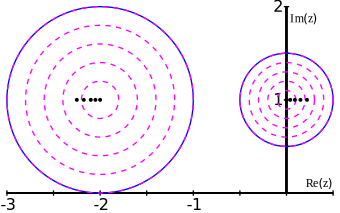
\includegraphics{Gershgorin_2.eps}}
\end{center}
\caption{How eigenvalues move.}
\label{F:Gershgorin_2}
\end{figure}

Let $p(t,x)$ be the characteristic polynomial of $A(t)$. Note that these characteristic polynomials are functions of both $t$ and $x$. Since polynomials are continuous functions, their roots (the eigenvalues of $A(t)$) are continuous for $t \in [0,1]$ as well. Let $\lambda(t)$ be an eigenvalue of $A(t)$. Note that $\lambda(1)$ is an eigenvalue of $A$, and $\lambda(0)$ is one of the $a_{ii}$ and is therefore in $S$. We will argue that $\lambda(t)$ is in $S$ for every value of $t$ in $[0,1]$. Let $r_i$ be the radius of $D_i$ and let $D(t)_i$ be the Gershgorin disk of $A(t)$ with the same center as $D_i$ and radius  $r(t)_i = tr_i$. Let $S(t) = \cup_{1 \leq i \leq m} D(s)_i$. Since $r(s)_i \leq r_i$, it follows that $D(s)_i \subseteq D_i$ and so $S(t) \cap S' = \emptyset$ as well. From topology, we know that since the disks $D_i$ are closed, the union $S$ of these disks is also closed. Similarly, $S(t)$ and $S'$ are closed. Thus, $\lambda(t)$ is continuous in a closed set and so does not leave the set. Thus, $\lambda(t)$ is in $S$ for every value of $t$ in $[0,1]$. 

\end{proof}

